\chapter{Geostrophic balance and coastal flow}
\label{chap:geostrophic}

\includegraphics[width=6.5in]{figs/Geostrophic/HaidaEddy}

\section{Geostrophic balance}

The second balance that involves the Coriolis force is the \Wikiref{Geostrophic balance}, and is when the Coriolis force is in ``balance'' with the pressure gradient:

\begin{equation}
    \frac{du}{dt} = \overunderbraces{\br{2}{geostrophic}}
    {- \frac{1}{\rho_0}\frac{dP}{dx} & +fv & + \frac{1}{\rho}\frac{d\tau_{xz}}{dz}}
    {&\br{2}{Ekman}}
\end{equation}
\begin{equation}
    \frac{dv}{dt} = \overunderbraces{\br{2}{geostrophic}}
    {- \frac{1}{\rho_0}\frac{dP}{dy} & -fu & + \frac{1}{\rho}\frac{d\tau_{yz}}{dz}}
    {&\br{2}{Ekman}}
\end{equation}
\begin{marginfigure}
    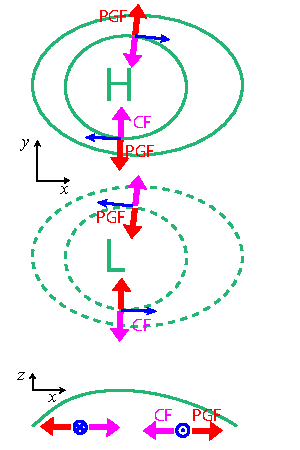
\includegraphics{figs/Geostrophic/BalanceSketch}
    \caption{Sketch of geostrophic force-balance for a sea-level high and a sea-level low in the northern hemisphere, looking from above, and from the south for the high.  The flow will be clockwise around a hight and counter-clockwise.}
    \label{fig:BalanceSketch}  
\end{marginfigure}
in which case the equations of motion simplify to:
\begin{eqnarray*}
    -\frac{1}{\rho_0}\frac{dP}{dx} & \approx & -fv\\
    -\frac{1}{\rho_0}\frac{dP}{dy} & \approx & +fu\\    
\end{eqnarray*}
In the northern hemisphere ($f>0$) this says that water turns to the right as in moves from high pressure to low.  This gives a clockwise circulation around an isolated high, or a counter-clockwise around an isolated low (\fref{fig:BalanceSketch})

Crucially, if we know the pressure gradient, we can directly calculate the geostrophic flow perpendicular to that pressure gradient from the equations above.  So, suppose the high in the cover figure is 16 cm, over 100 km.  The pressure difference due to this flow gives us an estimate of the velocity (assuming $f = 10^{-4}\ \mathrm{rad\,s^{-1}}$)
\begin{equation}
  |u| = \left|\frac{1}{f\rho} \frac{dP}{dx}\right| = \frac{1}{f\rho}\frac{\Delta P}{\Delta x} = \frac{g}{f} \frac{\eta_C - \eta_E}{\Delta x} \approx 0.16 \ \mathrm{m\,s^{-1}}
\end{equation}

The equation applies everywhere in the fluid, and is only made complex by the presence of water with different densities making the flow have a pressure gradient that changes with depth.  An observation of this can be seen in \fref{fig:InteriorEddy}, where there is a sea-surface high in the middle, but the pressure gradient inside the eddy is the other direction.  This causes the pressure gradient force to decrease with depth, and hence the geostrophic flow decays with depth as well. 

\begin{figure}
\begin{center}
    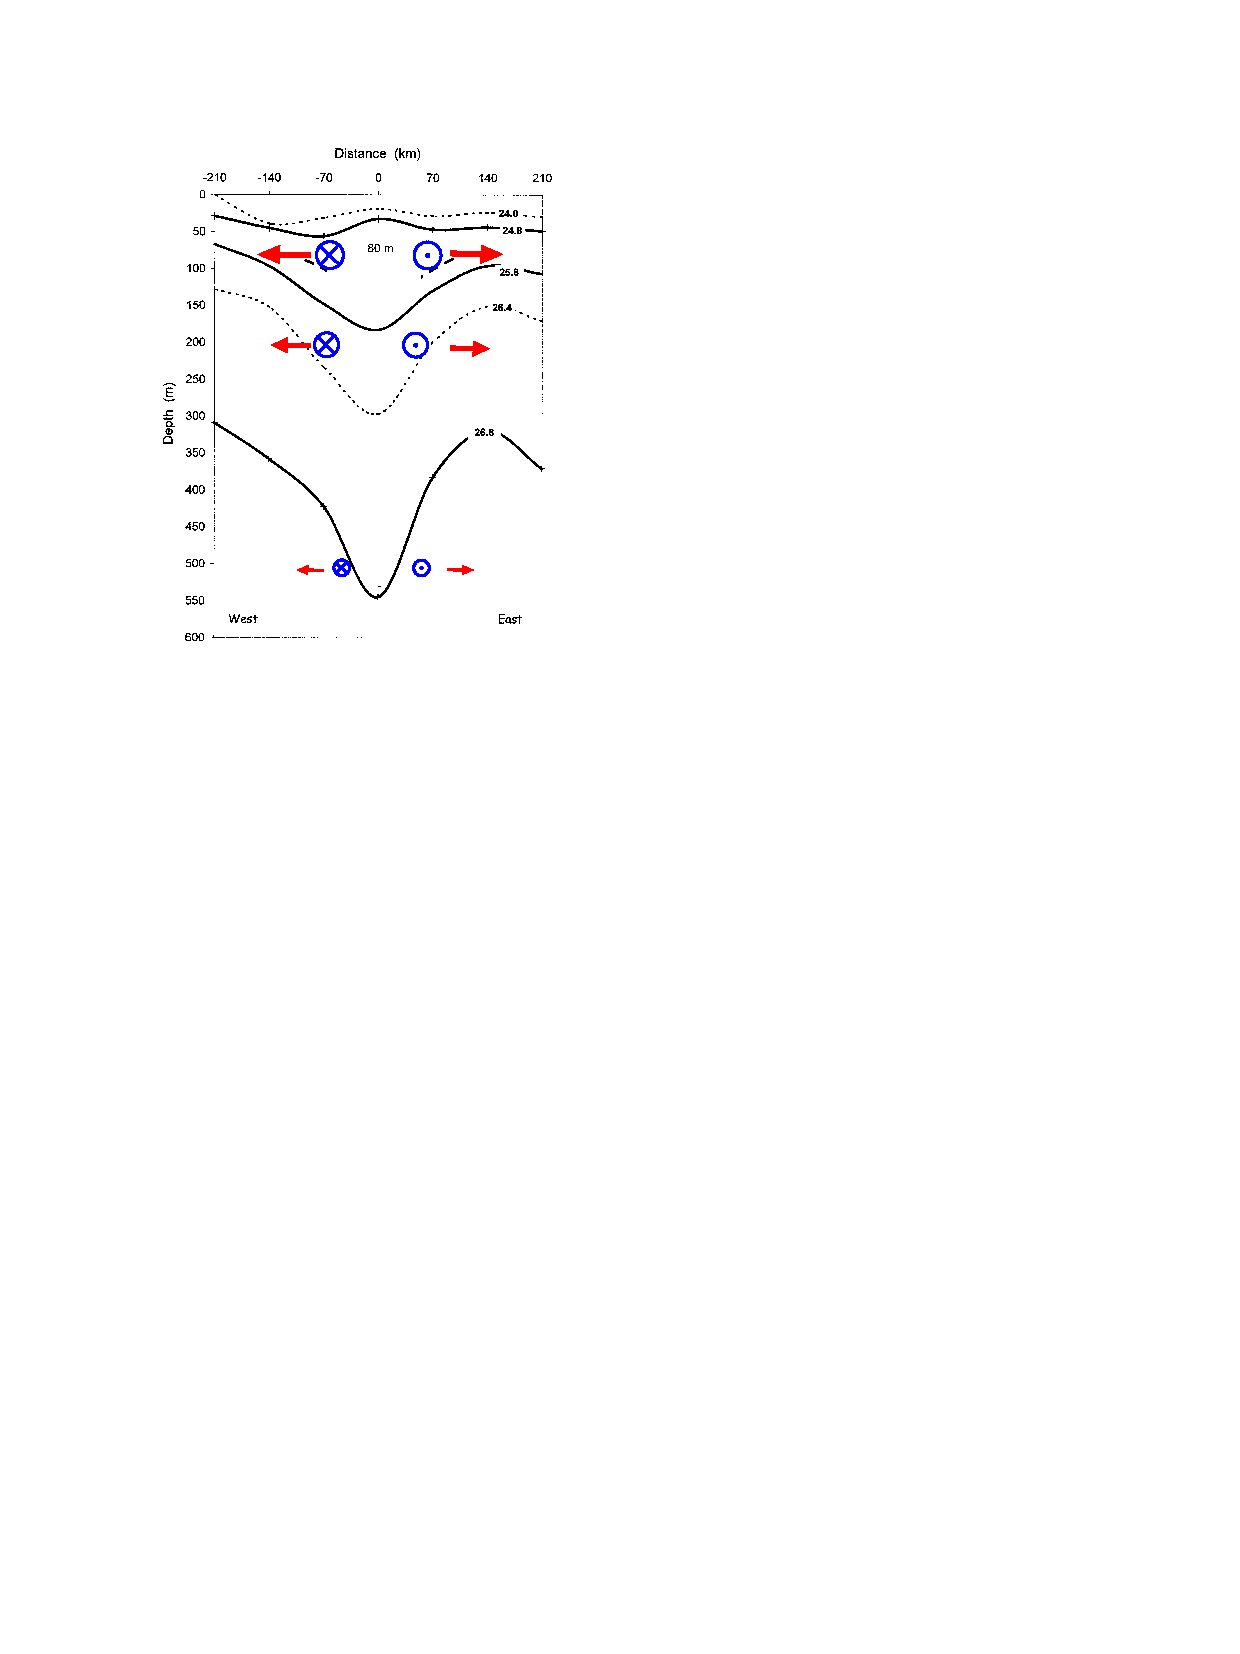
\includegraphics[width=2in]{figs/Geostrophic/InteriorEddy}
    \caption{Observations of density inside an Eddy.  Note how the density contours tend to counteract the high sea-surface height.  Blue circles with crosses are into the page, and with dots are out of the page, and the size is sketched to be proportional to the speed of the flow.}
    \label{fig:InteriorEddy}  
\end{center}
\end{figure}

As discussed in \fref{chap:EquationofState}, calculating the pressure gradient is simply a matter of calculating the pressure at two locations, and differencing, where the pressure is given by:
\begin{equation}
  P(z) / \rho_0 = \frac{1}{\rho_0}\int_z^\eta \rho g\ \mathrm{d}z \approx g\eta + \frac{1}{\rho_0}\int_z^0 \rho g\ \mathrm{d}z
\end{equation}
So imagine one flank of the eddy, and that the eddy is made of two densities $\rho_1 < \rho_2$ (\fref{fig:CounterPressure}).  In the upper layer 
\begin{equation}
  -\frac{1}{\rho_0} \frac{dP}{dx}(z=z_1) = -\frac{1}{\Delta x} g (\eta_B - \eta_A).
\end{equation}
In the lower layer, things are a bit more complicated, so we just do it step by step:
\begin{equation}
  P_A(z=z_2) = \rho_1 g (\eta_A - Z_A) + \rho_2 g (Z_A - z_2)
\end{equation}
\begin{equation}
  P_B(z=z_2) = \rho_1 g (\eta_B - Z_B) + \rho_2 g (Z_B - z_2)
\end{equation}
So the total pressure gradient in the lower layer is approximated as 
\begin{equation}
  -\frac{1}{\rho_0}\frac{P_B - P_A}{\Delta x} = \overbrace{-\frac{1}{\Delta x} g (\eta_B - \eta_A)}^{Surface} - \overbrace{\frac{1}{\Delta x} g \frac{\left(\rho_2 - \rho_1\right)}{\rho_0} (Z_B - Z_A)}^{Internal}
  \label{eq:InternalExternal}
\end{equation}

According to the geostrophic balance, then, the flow in the upper layer is into the page, and the one in the bottom layer is either into the page, but more slow, or even out of the page.  

\begin{figure}[hbt]
  \begin{center}
    \includegraphics{figs/Geostrophic/CounterPressure}
    \caption{Two-layer approximation of pressure gradients in an eddy.}
    \label{fig:CounterPressure}  
  \end{center}
\end{figure}

\subsection{Thermal wind}

The example above makes it clear that lateral density differences can drive velocity differences in the vertical if the flow is in geostrophic balance.  This can easily be extended to the continuous case with some  manipulation of the momentum equations.  If we take the vertical derivative of the x- and y-momentum equations we arrive at:
\begin{eqnarray}
    -\frac{1}{\rho_0}\frac{d^2 P}{dx dz} & = & -f \frac{dv}{dz} \\
    -\frac{1}{\rho_0}\frac{d^2 P}{dy dz} & = & f \frac{du}{dz} 
\end{eqnarray}
but $P = \int_z^{\eta}\rho g \mathrm{d}z$,  so we get the \Wikiref{thermal wind} relation.
\begin{eqnarray}
    -\frac{1}{\rho_0}\frac{d \rho}{dx} & = & -f \frac{dv}{dz} \\
    -\frac{1}{\rho_0}\frac{d \rho}{dy} & = & f \frac{du}{dz} 
\end{eqnarray}
so, if we know the horizontal pressure gradient, we can immediately say how the velocity changes with depth (though we do not know the absolute velocity).  

\subsection{Level of no motion and ``dynamic height''}

Back in the pre-satellite days, all oceanographers would have would be measurements of the density under the ocean, like those in \fref{fig:InteriorEddy}.  Estimating the sea-surface height was impossible; imagine detecting 15 cm over 100 km in an ocean that is otherwise also moving due to tides, surface waves, relative to a poorly-constrained geoid.  However, oceanographers noted that most ocean currents, like the eddy, had tilted density surfaces, and that the currents at depth go to approximately zero.  

Under these assumptions, oceanographers would assume that the pressure gradient at a ``level of no motion'' was zero, so that the geostrophic flow was zero there as well. In order to get this level of no motion the  pressure  gradients inferred from the interior density measurements were assumed to be balanced by a pressure gradient from the surface at that depth.  So, for instance, in the simple two-layer case the \fref{eq:InternalExternal}, the \emph{Surface} term was equal and opposite in sign to the \emph{Internal} term, if the deep layer was assumed to be not moving.  Note that this allows an estimate of the surface pressure gradient, and using the geostrophic balance, the surface velocities.  This surface pressure gradient is of course supplied by the sealevel interface being tilted, and  calculating these gradients is like calculating a ``dynamic height'' of the ocean.  

An example in \fref{fig:DynamicHeight}, calculated in the 1980s looks strikingly similar to the sea surface heights in \fref{chap:winddriven}.  In particular, where there is Ekman convergence in the subtropics there is a high of up to 2 m, and a low in the sub-polar regions where there is Ekman divergence.  The highs and lows are displaced to the west sides of the basins.  The steepest change in dynamic height correspond to the strongest currents, again largely concentrated on the west side of the basins, and associated with the Gulf Stream, Kurishio, East Australian current etc.  

\begin{figure}[hbt]
  \begin{center}
    \includegraphics{figs/Geostrophic/DynamicHeight1500}
    \includegraphics{figs/Geostrophic/DynamicHeight2500}
    \caption{Dynamic height with a level of no motion at 1500 m (top) and 2500 m (bottom).  Note these are quite similar, strongly indicative that the dynamics are largely above these depths.  }
    \label{fig:DynamicHeight}  
  \end{center}
\end{figure}

Just to summarize again how this is done:
\begin{enumerate}
    \item An interior pressure gradient is calculated at two ``stations'' as a function of depth using the density data from CTDs or other measurements.
    \item At a ``depth of no motion'' the pressure gradient is assumed to be zero, so a surface pressure gradient is added to the two points to make that be the case.
    \item If there are multiple stations in a line the surface pressure gradient is integrated to make a dynamic height with an arbitrary zero at some location. 
\end{enumerate}
 
We will come back to \emph{why} the dynamic height looks the way it does in the next chapter.

\section{Coastal upwelling, complete picture}

Using the Ekman and geostrophic balances we are now in a position to explain the coastal upwelling example in detail (i.e. \fref{fig:PerlinFig3a}, one snapshot in detail in \fref{fig:ShelfDetail}). 

\begin{figure}[hbt]
  \begin{center}
    \includegraphics{figs/Geostrophic/ShelfDetail}
    \caption{Data from \fref{fig:PerlinFig3a}.}
    \label{fig:ShelfDetail}  
  \end{center}
\end{figure}

First, the wind starts to blow towards the south; this sets up a southwards windstress $\tau_y^w$ (\fref{fig:CoastalStep1}, red circle).  When this flow is in a steady-state Ekman balance there will be an equal and opposite Coriolis force to the north (\fref{fig:CoastalStep1}, magenta circle).  That implies an offshore Ekman transport to the west given by 
\begin{equation}
  u_{Ek}D = \frac{\tau_y^w}{\rho_0 f}
\end{equation}


\begin{figure}[hbt]
  \begin{center}
    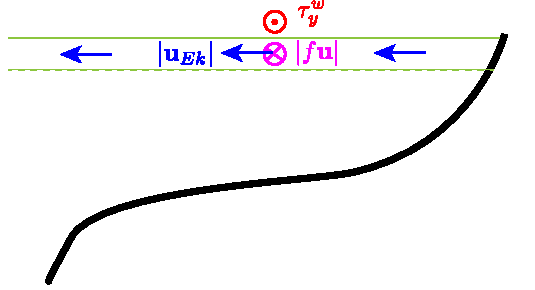
\includegraphics[width=2.85in]{figs/Geostrophic/CoastalStep1}
    \caption{On a continental slope, initially at rest, a wind stress blows from north to south (dotted red circle)}
    \label{fig:CoastalStep1}  
  \end{center}
\end{figure}

The offshore Ekman transport drops the sealevel at the coast (\fref{fig:CoastalStep2}, surface interface).   This creates a surface pressure gradient force that acts to push water back towards the coast (\fref{fig:CoastalStep2}, red arrow).  Again, in \emph{steady state} geostrophic balance, the pressure gradient force is balanced by a Coriolis force offshore, which must be generated by a geostrophic velocity to the south.  Note that this evolves in time with the deep water \emph{initially} moving onshore, but then being turned south (to the right) by the Coriolis force.  

\begin{figure}[hbt]
  \begin{center}
    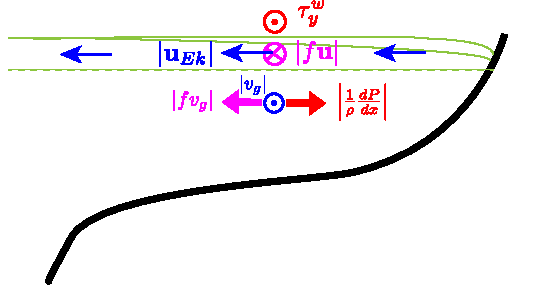
\includegraphics[width=2.85in]{figs/Geostrophic/CoastalStep2}
    \caption{After the Ekman transport has been active for a while, the sea level drops at the coast (green surface), and an interior geostrophic balanced flow is set up.}
    \label{fig:CoastalStep2}  
  \end{center}
\end{figure}

At this point the flow cannot be in steady state because we are transporting water offshore in the surface Ekman layer, but not having any onshore transport to replace it.  Without this return flow, the sea surface will continue to increase its tilt.  The return flow happens in the bottom Ekman layer.  The interior geostrophic flow moves south, so there is a corresponding bottom stress to the north $\tau_y^B$(\fref{fig:CoastalStep3}, red circle at bottom).  In a steady Ekman balance, this implies a Coriolis force to the south, which implies a net Ekman transport onshore (\fref{fig:CoastalStep3}, blue arrows, bottom), given by 
\begin{equation}
  u_{Ek}D = \frac{\tau_y^B}{\rho_0 f}
\end{equation}

The offshore Ekman transport drops the sealevel at the coast (\fref{fig:CoastalStep3})
\begin{figure}[hbt]
  \begin{center}
    \includegraphics[width=2.85in]{figs/Geostrophic/CoastalStep3}
    \caption{}
    \label{fig:CoastalStep3}  
  \end{center}
\end{figure}

When is the whole flow balanced?  When $\tau^B = \tau^W$ so that the transport in the bottom Ekman layer is the same as the transport in the surface Ekman layer.  So, if we know the wind stress, and have a good estimate of the bottom \Wikiref{drag co-efficient}, $C_D\approx10^{-3}$, then we can guess what the mean geostrophic velocity is, and hence the size of the sea surface tilt.  For the Oregon shelf, $\tau_y^W\approx -0.15\ \mathrm{N\,m^{-2}}$ (minus means to the south).  Than means that the geostrophic velocity $v_g \approx 0.35\ \mathrm{m\,s^{-1}}$ in order for $\rho_0 C_D |v_g|^2$ to be large enough to provide the bottom stress to match.  This is approximately the same as the observations near the bottom.  

We can further calculate the sea-surface height drop across the 20-km width of the shelf from $g \frac{d\eta}{dx} = f v_g$ or $\Delta \eta =  0.08\ \mathrm{m}$ across the shelf.  

\subsection{Internal dynamics on shelf}

The final thing we notice about the shelf observations is that the  flow is slower towards the sea-floor than at the surface.  This is also largely explained by the geostrophic balance.  Note that the isopycnals tilt up towards the coast, counteracting the surface pressure gradient (also sketched in \fref{fig:CoastalTilt}).  This means that the surface tilt is actually larger than we calculated above if the bottom velocity is to remain $0.38\ \mathrm{m\,s^{-1}}$, leading to faster velocities near the surface.  

\begin{figure}[hbt]
  \begin{center}
    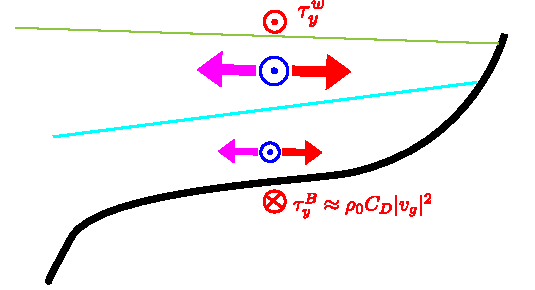
\includegraphics[width=2.85in]{figs/Geostrophic/CoastalTilt}
        \caption{Sketch of pressure gradient changes if there are titled isopycnals (cyan line) in the section, as observed in the coastal data.  The tilted isopycnal counteracts the surface tilt, slowing the barotropic flow.  }
    \label{fig:CoastalTilt}  
  \end{center}
\end{figure}

\clearpage
\section{Exercises}

\paragraph{Geostrophic balance two stations}

Calculate the geostrophic flow at two stations 50 km apart, assuming $f=10^{-4}\ \mathrm{rad\,s^{-1}}$.  
Approximate the density measured at each location as 50-m blocks of homogeneous density:

\begin{tabular}{l|cc}
  $z\ \mathrm{[m]}$ & $\rho_A \mathrm{[kg\,m^{-3}]}$ & $\rho_B \mathrm{[kg\,m^{-3}]}$ \\
  \hline
  0--50 & 1021& 1020 \\
  50--100& 1022& 1021\\
  100--150& 1024& 1023\\
  150--200& 1025& 1024\\  
\end{tabular}

\begin{itemize}
  \item If the surface pressure gradient is zero, what is the internal pressure gradient at 50, 100, 150, and 200 m? (do not drop too many decimal places!)
  \item What is the direction and strength of the \emph{geostrophic} velocity at the 4 depths?
  \item If there is a pressure gradient, what must its direction and strength be so that the geostrophic flow is zero at 200 m?
  \item How large must the surface difference be at the two stations? 
  \item What is the new flow at the other depths in the presence of this surface gradient?
\end{itemize}

\paragraph{Geostrophic flow Gulf Stream}

Consider the temperature section across the Gulf Stream (\fref{fig:GulfStreamExample}).  Assuming a level of no motion at approximately 1500 m, what does 
\begin{itemize}
    \item the sea-surface tilt look like?
    \item the interior velocity look like (just a sketch)?
    \item where would you expect the Gulf Stream to be the fastest?
\end{itemize}

\begin{figure}[hbt]
  \begin{center}
    \includegraphics[width=1.8in]{figs/Geostrophic/GulfStreamLoc}
    \includegraphics[width=2.7in]{figs/Geostrophic/GulfStreamTemp}
    \caption{Location of measurements in the Gulf Stream, and plot of temperature across the section \citep{johnsetal95}.}
    \label{fig:GulfStreamExample}  
  \end{center}
\end{figure}

